\documentclass[a4paper,12pt]{article}

\usepackage{fancyhdr}
\usepackage{lastpage}
\usepackage{amsmath}
\usepackage{tikz}
\usepackage{amsfonts}
\usepackage{graphicx}

\newcommand{\V}[1]{\ensuremath{\vec{#1}}}
\newcommand{\F}[2]{\ensuremath{\frac{#1}{#2}}}
\newcommand{\Q}[1]{\newpage \section*{#1}}
\newcommand{\acc}[1]{\overset{..}{#1}}
\newcommand{\vel}[1]{\overset{.}{#1}}


\pagestyle{fancy}
\lhead{Samuel Loomis}
\setlength{\headheight}{15pt}
\chead{Classical Mechanics HW 1}
\rhead{13 November 2013}
\lfoot{}
\cfoot{\thepage\ of \pageref{LastPage}}
\rfoot{}

\begin{document}

\section*{Problem 1}
A parallel plate capacitor is formed by two circular plates of area $A$ and placed at a distance $d$ apart. It is connected with two inter-winding circular coils. The coils have the same radius $a$ and total length $l$ but different density of wires: $n_r$ and $n_b$ rounds per unit length respectively.  Initially the capacitor has a charge Q, and the switch is closed at $t=0$. (1) How is the charge changing as a function of time? (2) Calculate the magnetic energy in the coil and the electric energy in the capacitor, how does the total change with time?  (3) Although there is no resistance in the circuit, people find the energy gradually getting lost, where does it go?  Use Poynting vectors to help your reasoning.\\ \\
\begin{figure}[h]
\centering
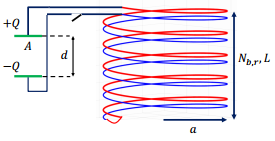
\includegraphics{Capacitor_Coil.png}
\end{figure}\\ \\
At time $t=0$ when the switch is closed, a current will begin to form.  When the switch is closed, the current will flow from the positive plate to the negative plate  and thus the positive current will be defined as top plate to bottom plate or according to the picture, clockwise in the wires near the capacitor.  The current that forms will be:
\[I=-\vel{Q}\]
The two solenoids will resist the change of current creating an emf value equal to the negative inductance value times the change in current:
\[\varepsilon_L=-L\vel{I}=L\acc{Q}\]
The total emf in this system has terms from both the solenoids and the capacitor:
\[\varepsilon=\varepsilon_C+\varepsilon_L=\F{Q}{C}+L\acc{Q}\]
The circuit doesn't include a resistor and thus the total emf must equal 0:
\[\F{Q}{C}+L\acc{Q}=0\]
Rewriting:
\[\acc{Q}=-\F{1}{LC}Q\]
Solution to this dif eq:
\[Q(t)=Q_0e^{-i\sqrt{\F{1}{LC}}t}\]
The inductance value is determined by a combination of the two solenoids. The current that forms will be the same in both the solenoids, however, the current through the red solenoid and the current through the blue solenoid will be in opposite directions.  The two solenoids can be thought of as a single solenoid with $(n_r-n_b)l$ total number of turns.  This works because any flux generated through a red loop will have equal and opposite flux generated through a blue loop.  The total will depend on one loop having more turns than the other.  \\
\\
The inductance of a solenoid is $L=\F{N\Phi}{I}$, where N is the total number of turns,A is the cross sectional area, and $\Phi$ is the total magnetic flux.  $\Phi=\mu_0\F{NIA}{L}$, this makes the inductance:
\[L=\mu_0\F{N^2A_L}{l}\]
The inductance of the modified solenoid is then:
\[L= \mu_0(n_r-n_b)^2lA_L\]
The capacitance of this capacitor is:
\[C=\F{\epsilon_0A_C}{d}\]
$Q(t)$ now becomes:
\[Q(t)=Qe^{-i\sqrt{\F{d}{\mu_0\epsilon_0(n_r-n_b)^2lA_LA_C}}t}\]
$A_L=\pi a^2$ and $A_C=A$ thus $Q(t)$ becomes:
\[Q(t)=Qe^{-i\sqrt{\F{d}{\mu_0\epsilon_0(n_r-n_b)^2l\pi a^2A}}t}\]
Solving for the magnetic energy in the coil:\\ 
\\
The magnetic energy $E_B$ is:
\[E_L=\F{1}{2}LI^2\]
The current is equal to the change of charge with respec to time or:
\[I=\vel{Q}=-iQ\sqrt{\F{d}{\mu_0\epsilon_0(n_r-n_b)^2l\pi a^2A}}e^{-i\sqrt{\F{d}{\mu_0\epsilon_0(n_r-n_b)^2l\pi a^2A}}t}\]
The magnetic energy is then:
\begin{align*}
E_L&=-\F{1}{2}LQ^2\F{d}{\mu_0\epsilon_0(n_r-n_b)^2l\pi a^2A}e^{-2i\sqrt{\F{d}{\mu_0\epsilon_0(n_r-n_b)^2l\pi a^2A}}t}\\
&=-\F{1}{2}Q^2\F{d}{\epsilon_0A}e^{-2i\sqrt{\F{d}{\mu_0\epsilon_0(n_r-n_b)^2l\pi a^2A}}t}
\end{align*}
The energy of the capacitor is:
\[E_C=\F{1}{2}\F{Q^2(t)}{C}=\F{1}{2}Q^2\F{d}{\epsilon_0A}e^{-2i\sqrt{\F{d}{\mu_0\epsilon_0(n_r-n_b)^2l\pi a^2A}}t}\]
The total energy is:
\[E_L+E_C=0\]
The  Poynting vector is $\F{1}{\mu_0}\V{E}\times\V{B}$ , at every point on the solenoids, $\V{E}\times\V{B}$ points out of the solenoid.  This means that the energy is escaping the solenoid in the form of electromagnetic radiation.


\Q{Problem 2}
Same configuration as Problem 1.  Now if an electron escaped from the capacitor at $t=0$ with zero velocity, describe its trajectory as a function of $t$. If you can not solve for the trajectory, make sure you have the right equations. Even though we may not be able to solve for the equations, there are several categories of trajectories and extreme cases you can physically anticipate, try to list them and explain.
\\
\\
Looking at this analytically...  An electron escaping one of the plates of the capacitor will be influenced by the electric field in place and then as it picks up velocity, the magnetic field plays a role.  The force felt by the electron will be $F=q(\V{E}+\V{v}\times\V{B})$.  The E field will accelerate the electron in the oposite direction it is heading, and as such the electron will develop an oscillation between the plates.  If the electron came out at the center of the capacitor plate, the motion would be entirely vertical(z direction only with the z axis running from the center of one plate to the center of the other)... this is because the B field is dependant on r from the center of the plate. If the electron started any arbitrary distance away from the center of the plate, the B field would then push it in a $-v\times B$ direction.  As the E field increases in the positive z direction, looking down from above, the B field will curl counter clockwise.  The velocity will begin to form in the direction of $\V{E}$ and $\V{v}\times\V{B}$ will be radially outward. If the E field is still growing in the positive z direction, the electron will gain a stronger and stronger acceleration in the negative z direction, however, the positive change in E will be getting lesser and thus the B field will be getting weaker, untill the electric field is maximum and for a brief moment the magnetic field goes away.  The E field will then begin to decrease and will cause the magnetic field to begin growing in the clockwise direction.  As this occurs, the electron will still be accelerated in the negative z direction and the magnetic field will accelerate the electron in the negative r direction.  As the electron gains velocity in the r direction, v cross B begins to push the electron in the positive z direction as well as in the negative r direction.  This appears to be an almost circular oscilation, depending on the strength of both the E field and the B field.
\\
\\
For $t=0$ the electric field starts at a maximum in the negative z direction.  The change in electric field will be in the positive z direction and thus the magnetic field, starting weak and growing stronger, will be in the clockwise direction.  If an electron hopped off the bottom plate the electron will experience a strong positive acceleration and once it starts moving, the growing magnetic field will bias the direction inward, and with an outward velocity begin to accelerate it up as well.  When the electric field becomes 0 and the magnetiv field is at a maximum, the only acceleration will be  from the B field and it should be inward and downish.  The magnetic field will begin to dwindle untill the E field is maximum and negative.  Where the B field will again go away and then a moment later grow in the counter clockwise direction.  The moment the E field becomes negative, the electron will begin getting a negative z direction.  The moment the magnetic field switches, the electron will experience a negative acceleration (inward and downish) from the magnetic field.  The direction of the velocity at any point in time ultimately judges how the electron accelerates due to $\V{B}$.
\end{document}


